% !TEX encoding = UTF-8 Unicode
% -*- coding: UTF-8; -*-
% vim: set fenc=utf-8
%\inputencoding{utf8}

\section{Uživatelské rozhraní}\label{sec:uživatelskéRozhraní}

Uživatelské rozhraní a jeho návrh se řadí do odvětví Interakce člověka a počítače (anglicky Human-computer interaction nebo HCI).
Jedná se složitou problematiku, která zahrnuje přístupnost, použitelnost a důvěryhodnost uživatelského rozhraní a to nejen pro webové aplikace.

\subsection{Material Design}\label{subsec:materialDesign}

Pro prototyp aplikace jsem se rozhodl využít již připravené zásady pro tvorbu uživatelského rozhraní od společnosti Google nazvané Material Design.
Tyto zásady jsou veřejně dostupné na stránkách společnosti Google a řeší výše zmíněnou problematiku návrhu uživatelského rozhraní.~\cite{google:md},~\cite{google:mdUsability}

Jako implementaci těchto zásad jsem využil knihovnu \texttt{Material-UI}.
Tato knihovna implementuje jednotlivé komponenty zmíněné v zásadách Material design jako React komponenty (více o knihovně React v sekci~\ref{subsec:reactjs}).

Použitím této knihovny vzniklo vizuálně příjemné a intuitivní uživatelské rozhraní (viz náhled rozhraní na obrázku~\ref{fig:uiScreenshot}).
Uživatelské rozhraní aplikace je navržené tak, aby šlo aplikaci snadno použít i na zařízeních s rozdílnou velikostí a poměrem obrazovky (je takzvaně responzivní).

\begin{figure}[ht!]
    \centering
    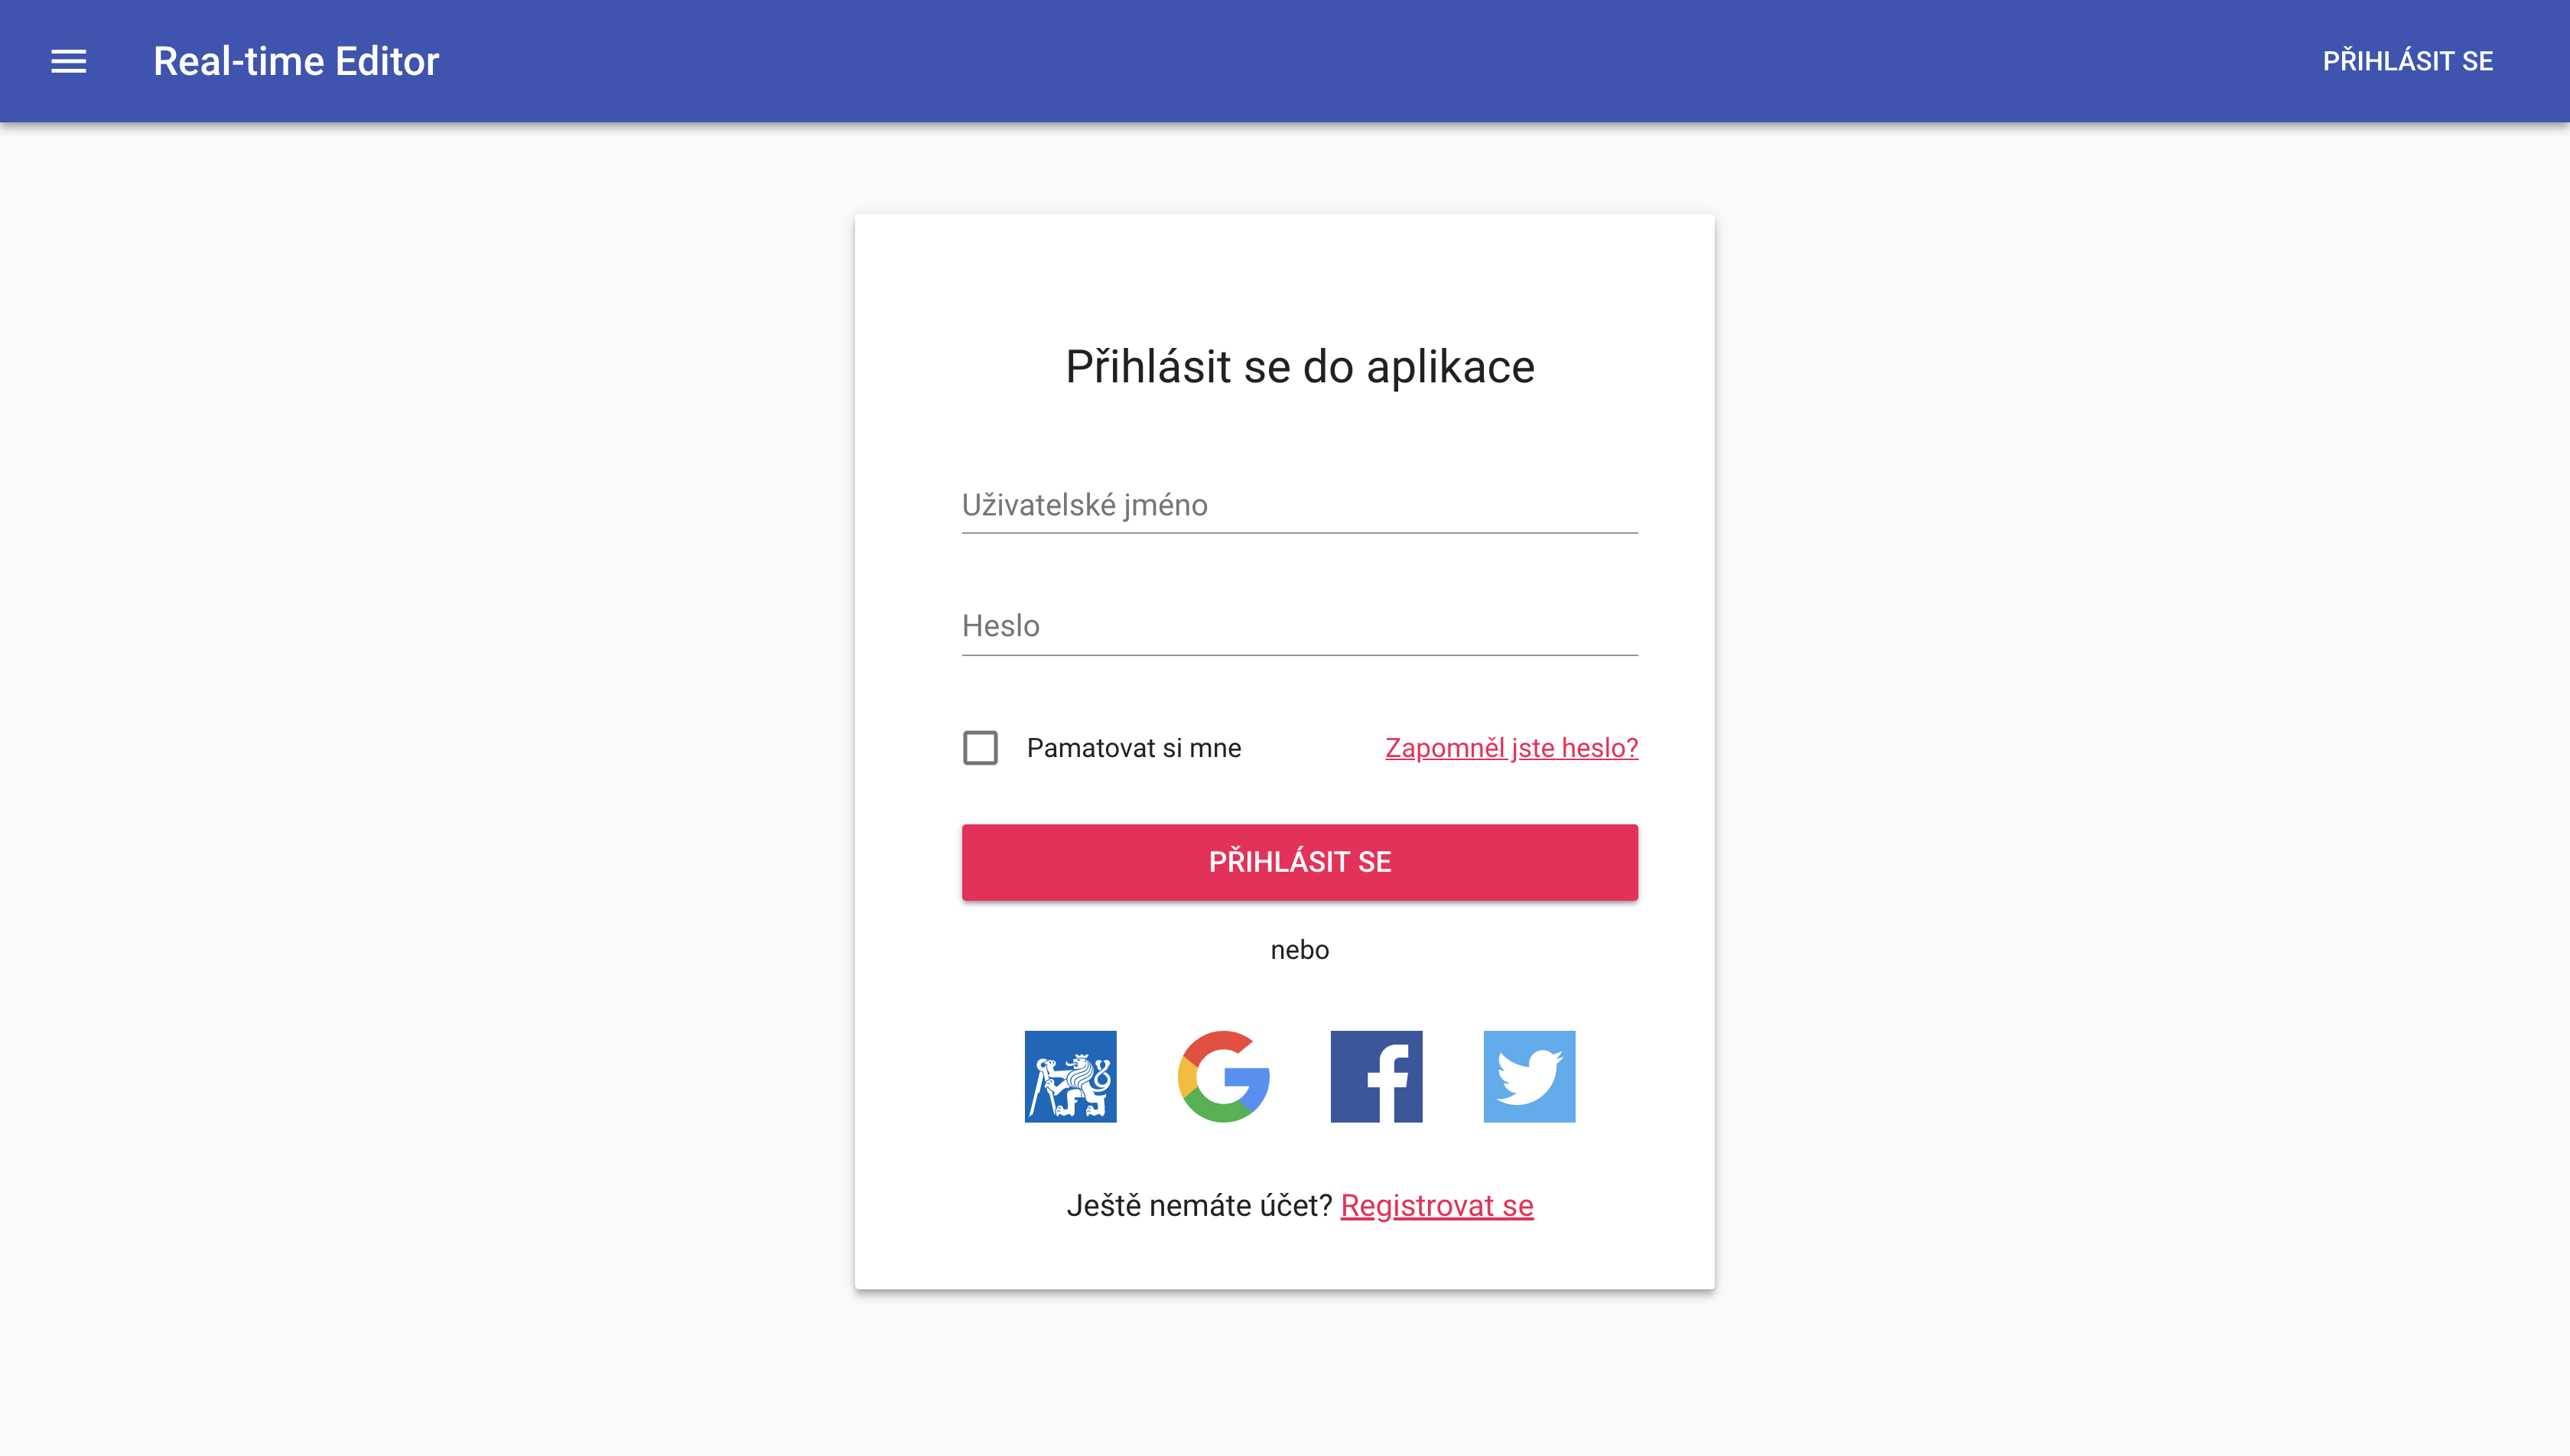
\includegraphics[width=\textwidth]{partials/realizace/uiScreenshotCZ.png}
    \caption{Náhled přihlašovací obrazovky prototypu aplikace}\label{fig:uiScreenshot}
\end{figure}

\subsection{Textový editor}\label{subsec:textovýEditor}

Textový editor je hlavní částí prototypu aplikace.
Z tohoto důvodu není vhodné použít jednoduchou textovou oblast a rozhodl jsem se proto použít komplexnější textový editor.

Pro implementaci textového editoru jsem použil JavaScriptovou (více o jazyce v sekci~\ref{subsec:javascript}) knihovnu \texttt{CodeMirror}.
Tato knihovna poskytuje pomocí svého \gls{API} rozsáhlé možnosti pro manipulaci textu, vzhledu, zvýrazňování syntaxe a celkového chování editoru~\cite{codemirror:docs}.
Jejím použití vznikl textový editor s rozsáhlými možnostmi nastavení a příjemným vzhledem (viz náhled editoru na obrázku~\ref{fig:uiEditor}).

\begin{figure}[ht!]
    \centering
    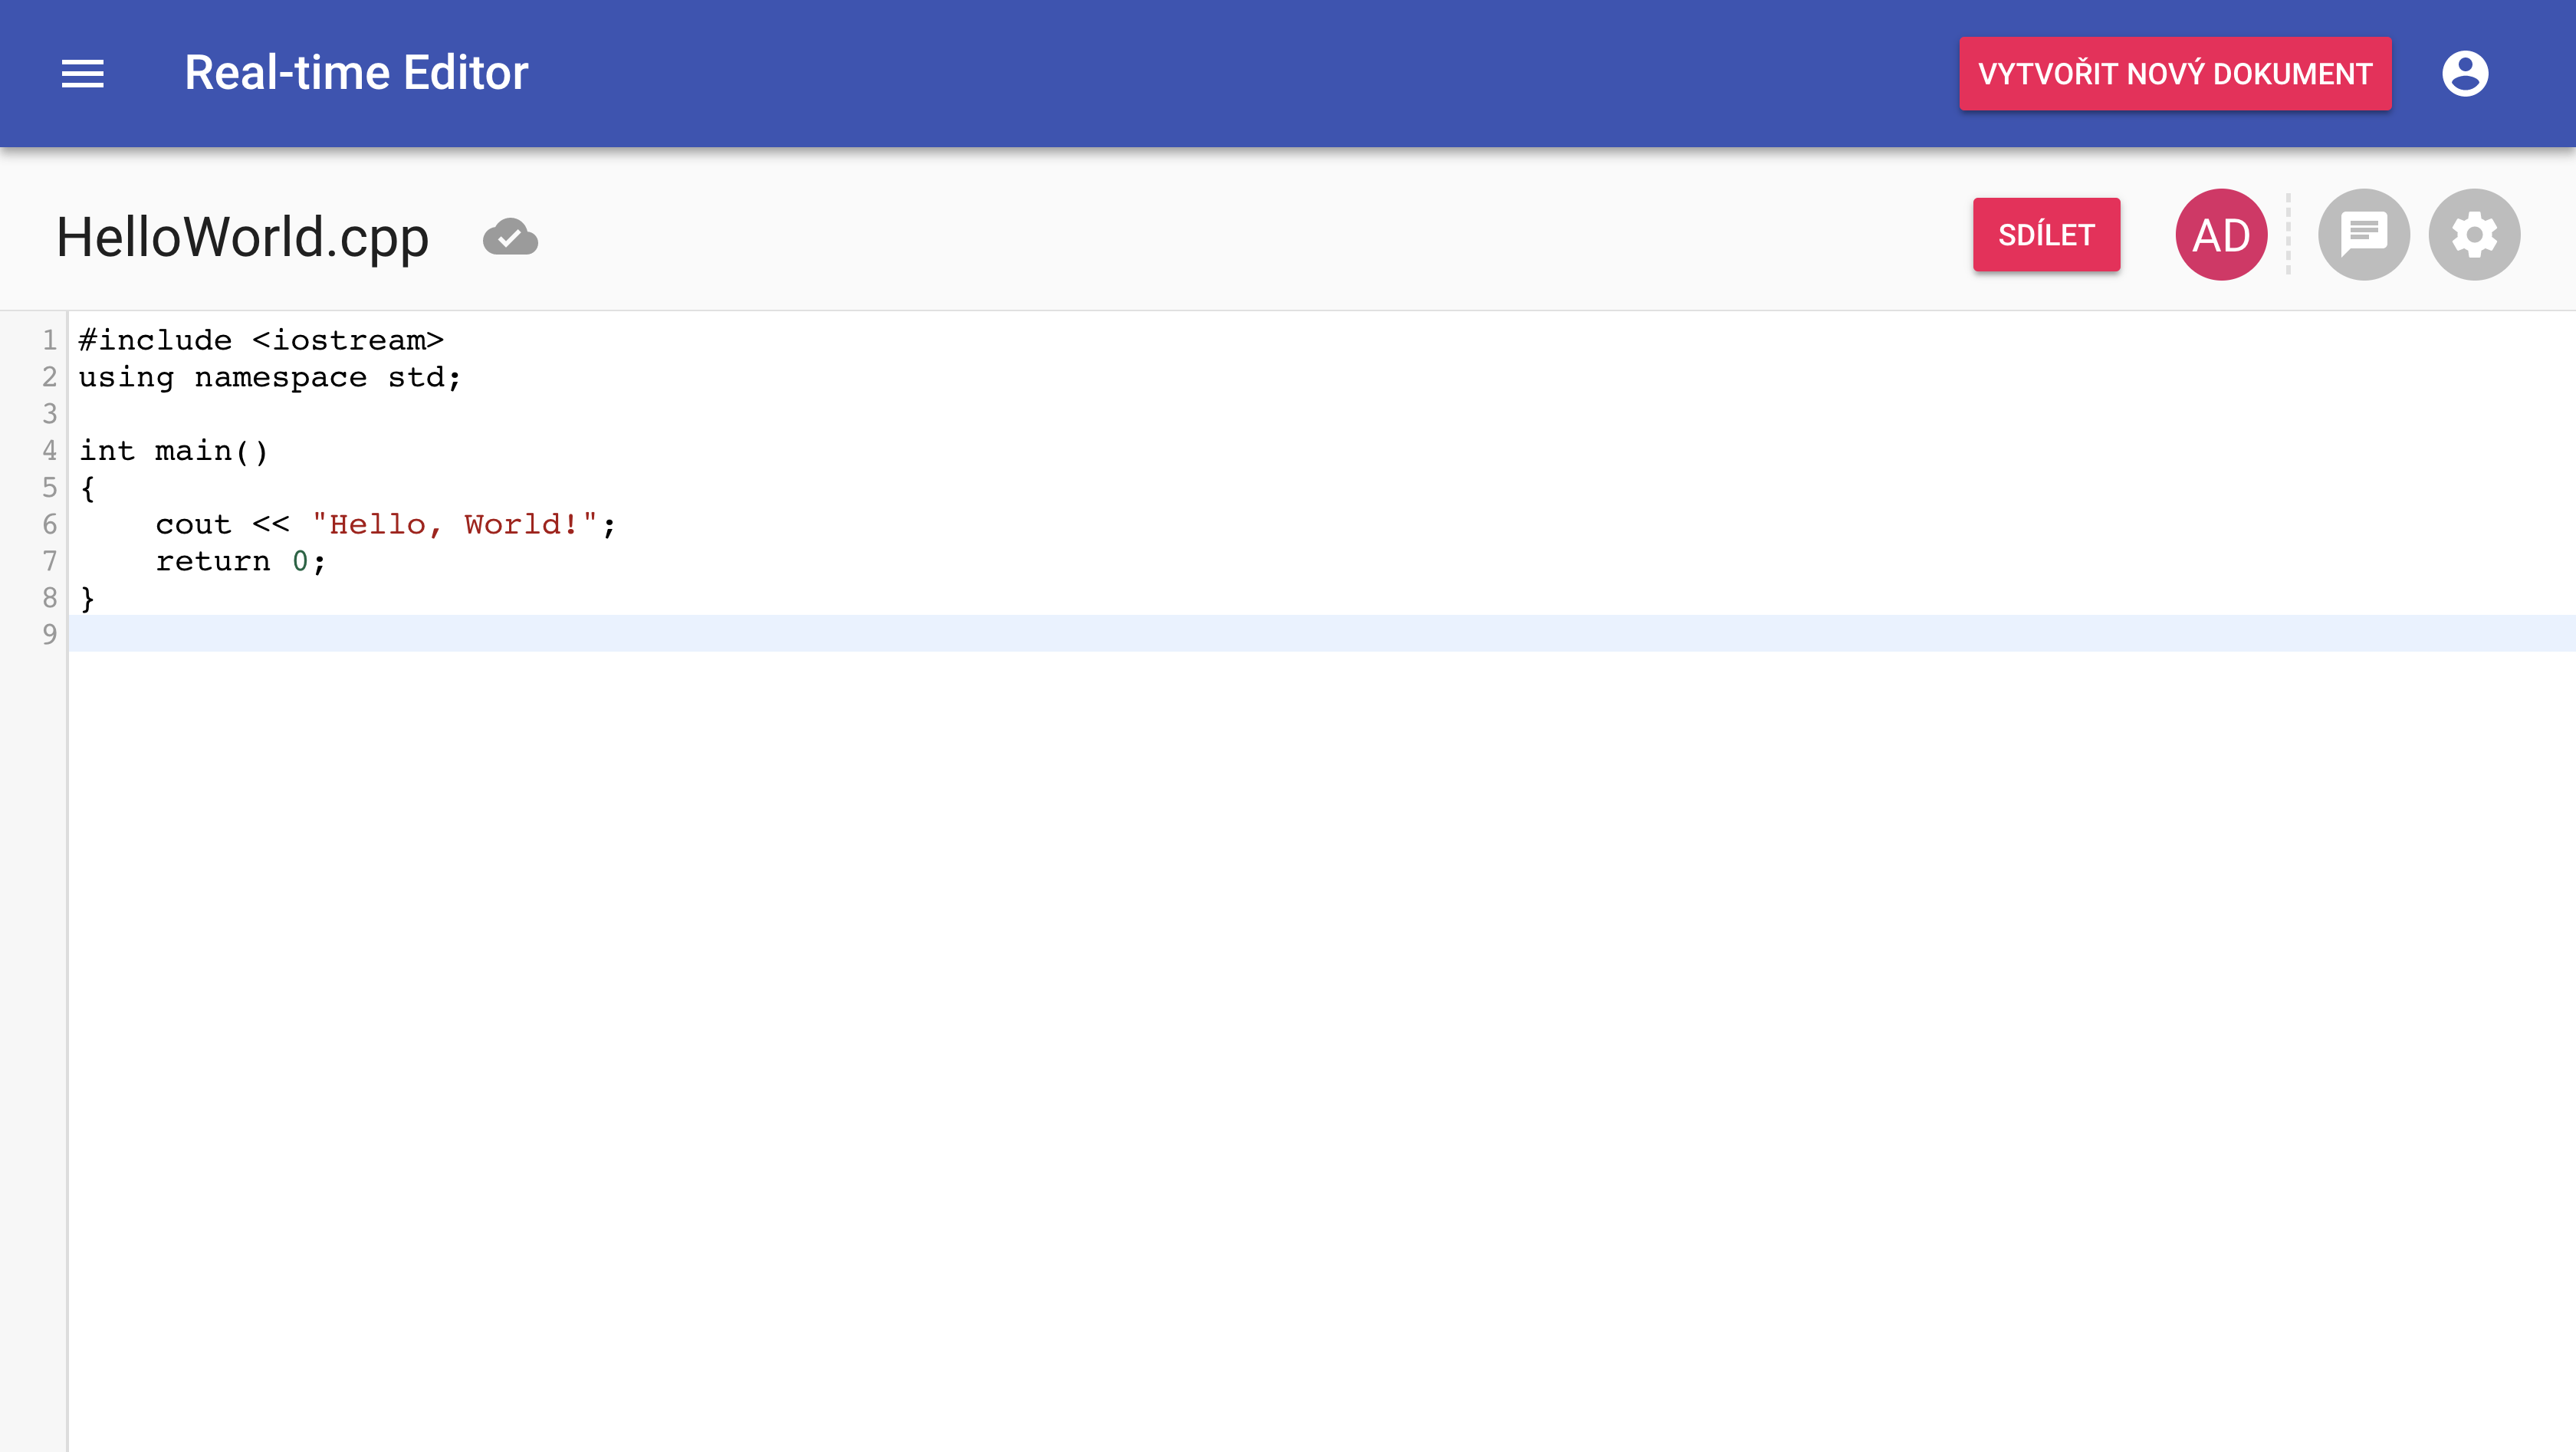
\includegraphics[width=\textwidth]{partials/realizace/uiEditor.png}
    \caption{Náhled editoru prototypu aplikace}\label{fig:uiEditor}
\end{figure}